%标题控制(caption、bicaption等宏包)
%并排与子图表(subcaption、subfig、floatrow等宏包)
%绕排(picinpar、wrapfig等宏包)

\documentclass{ctexart}
%\usepackage{ctex}

%支持格式EPS、PDF、PNG、JPEG、BMP
%语法:\includegraphics[keyvals]{imagefile}
\usepackage{graphicx}
%用于数学矩阵
\usepackage{amsmath}
%用于数学公式内的一些特殊符号
\usepackage{amssymb}
\graphicspath{{figures/}}%图片在image文件夹内

\begin{document}
	\section{插图}
	\LaTeX{}中的插图:
	
	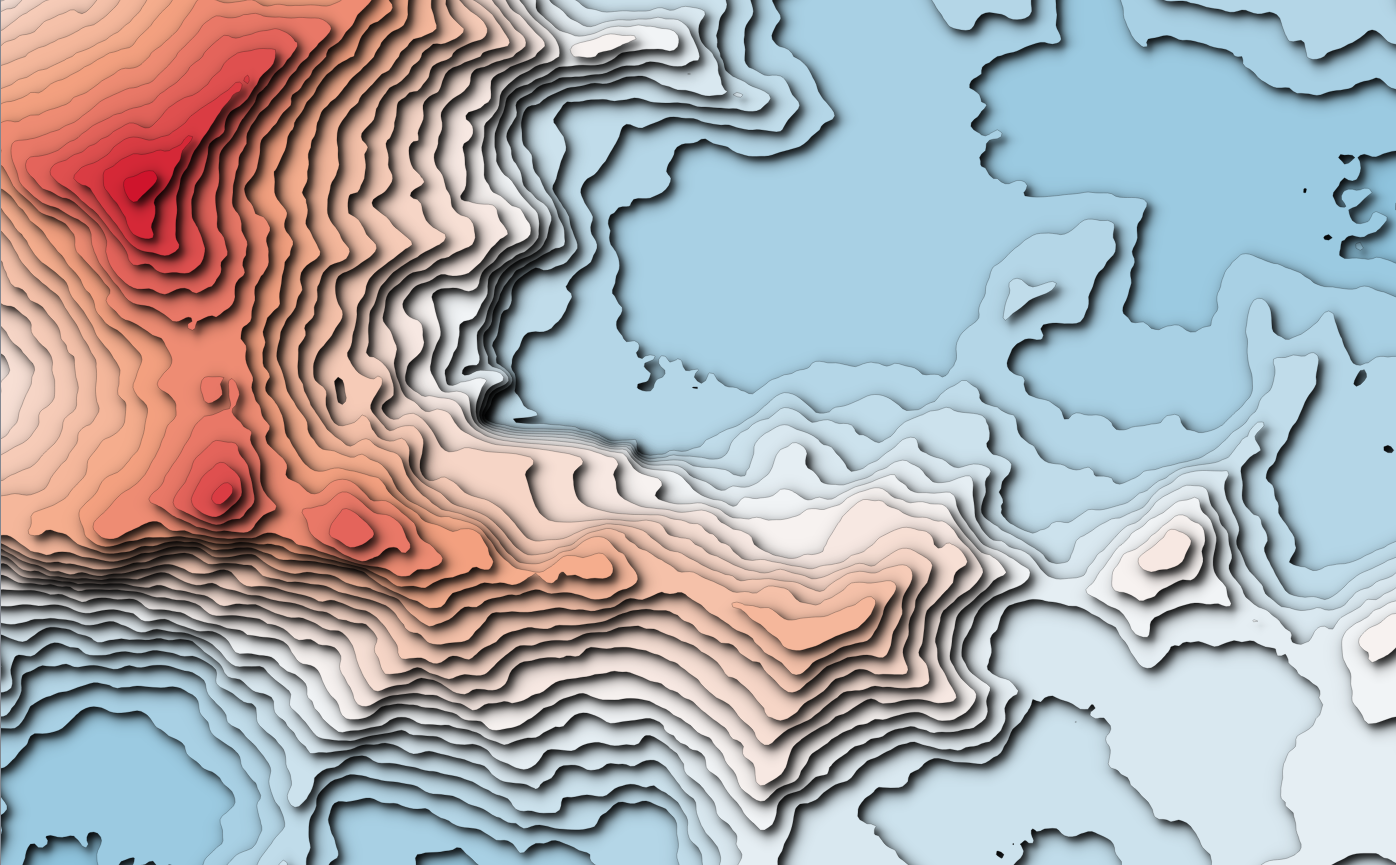
\includegraphics[scale=0.1]{test.png}
	
	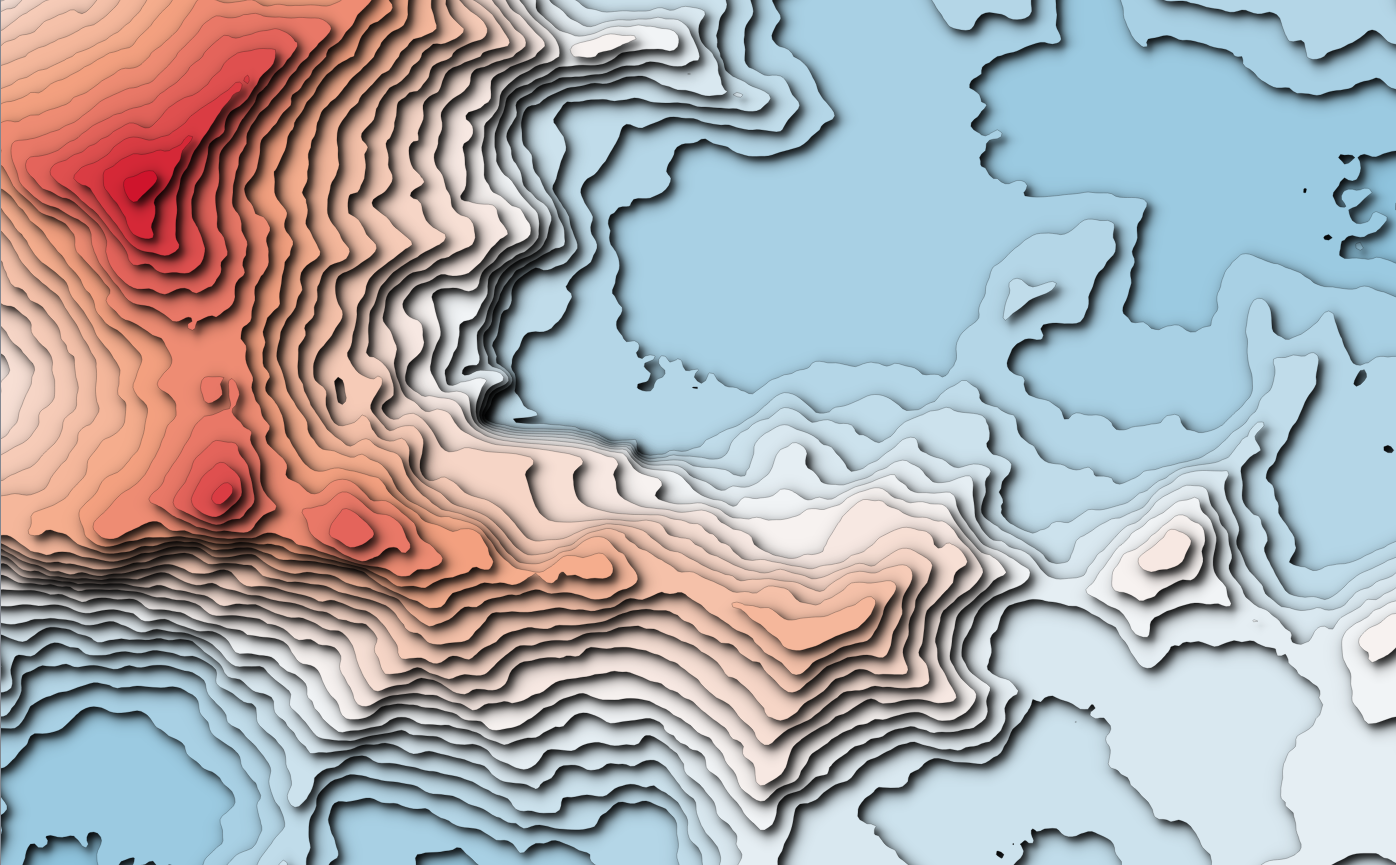
\includegraphics[height=2cm]{test.png}
	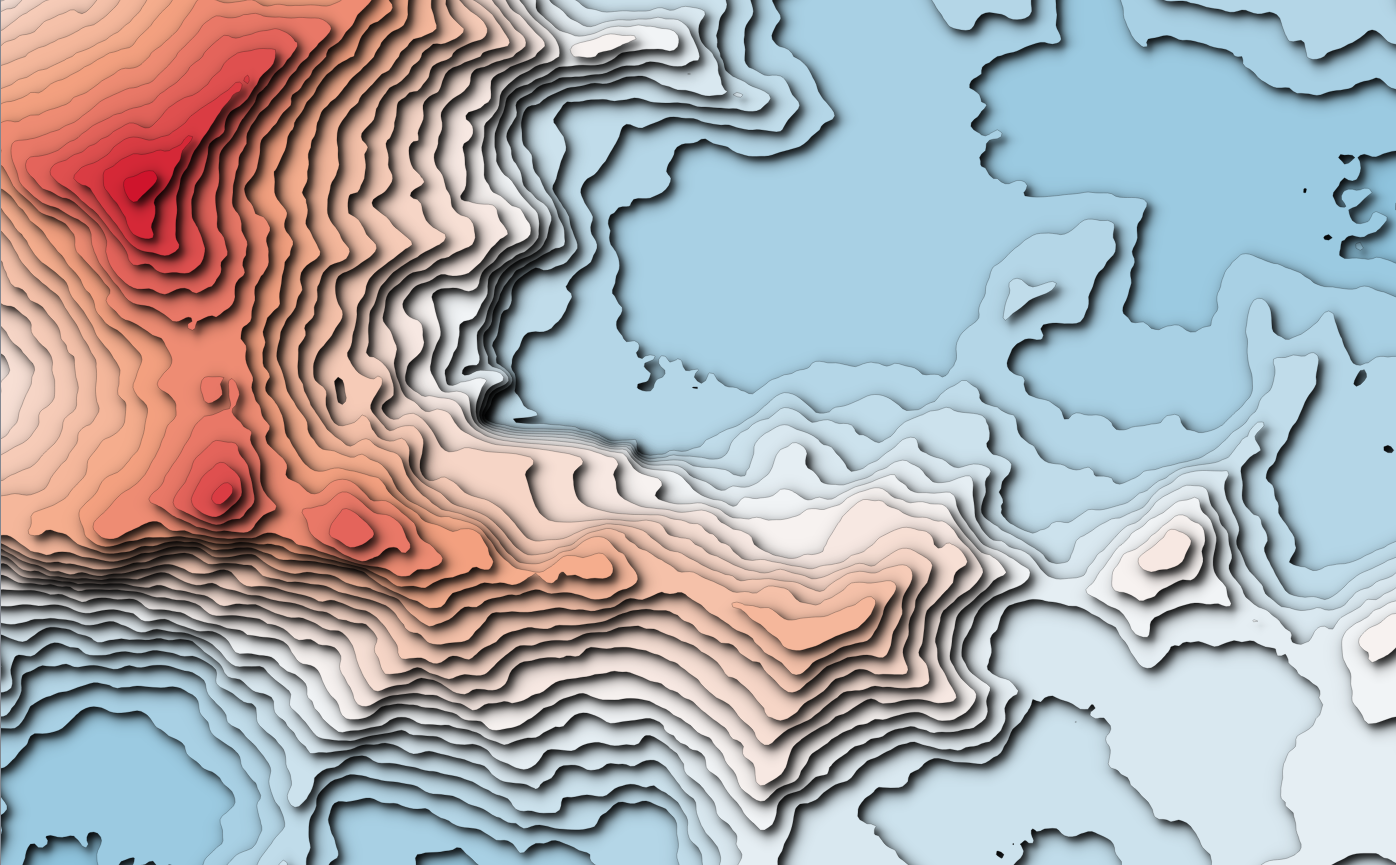
\includegraphics[width=2cm]{test.png}
	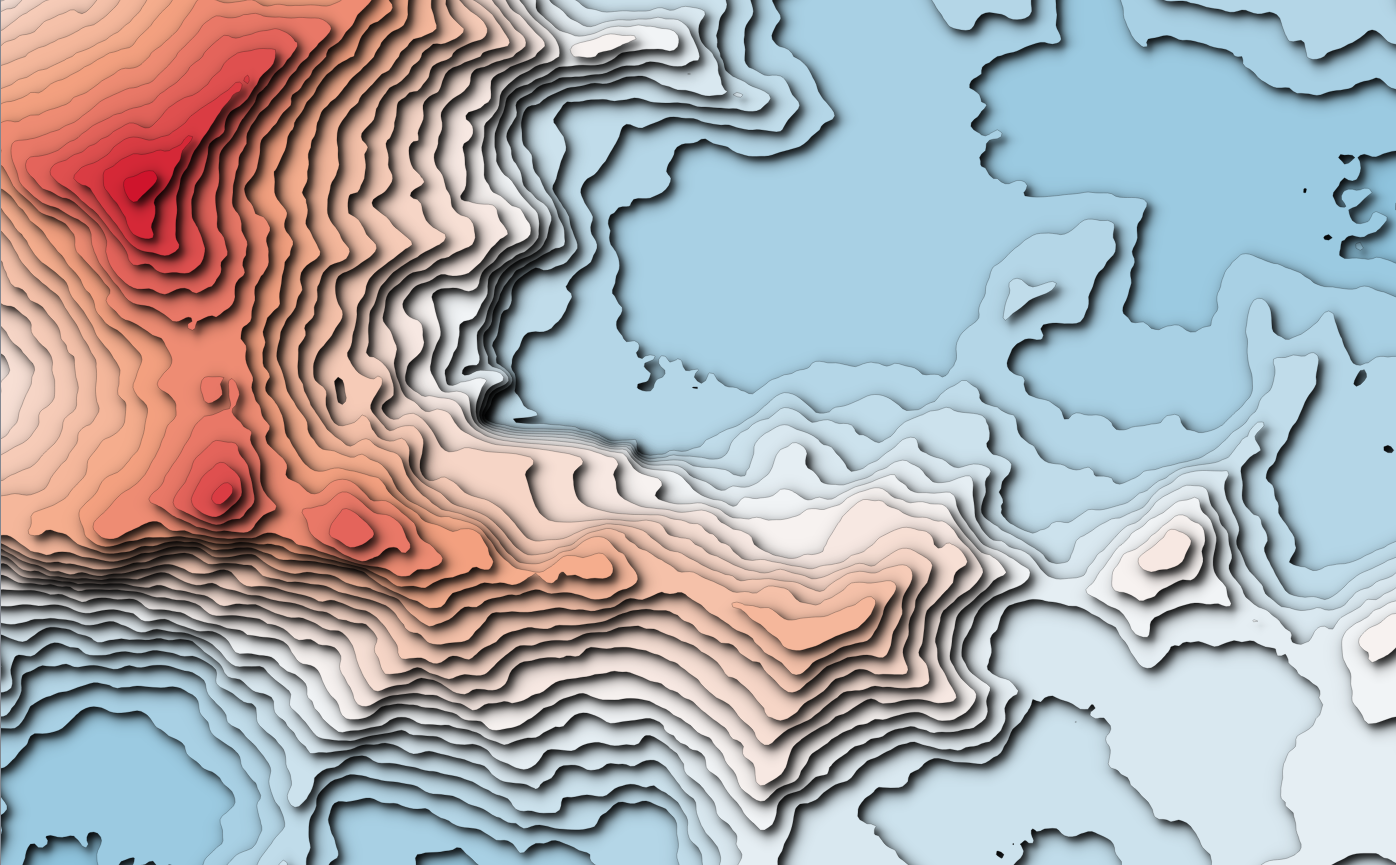
\includegraphics[width=2cm,height=2cm]{test.png}
	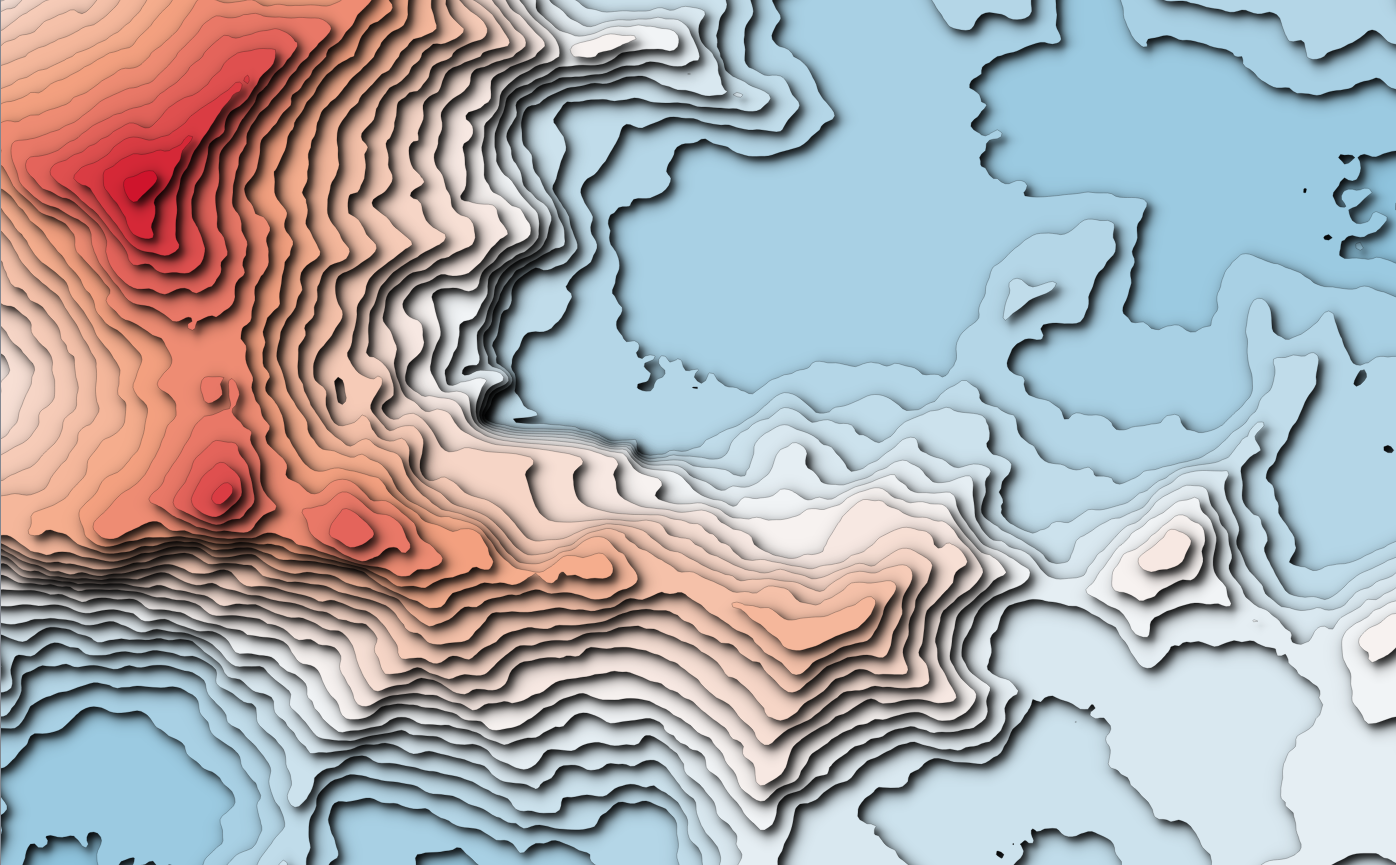
\includegraphics[angle=-45,width=2cm]{test.png}
	%textheight、textwidth是与文本相关的参考
	%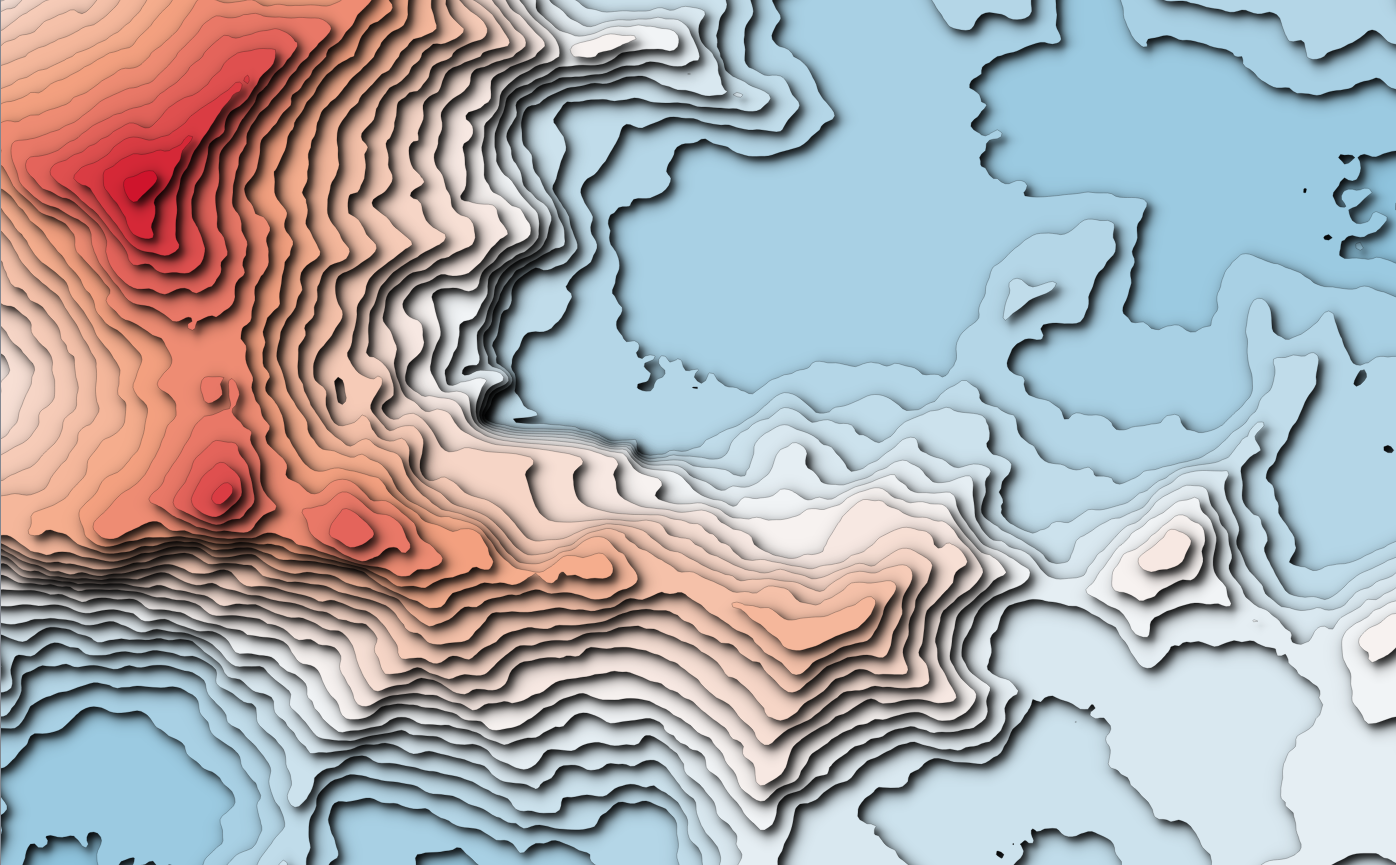
\includegraphics[height=0.1\textheight]{test.png}
	%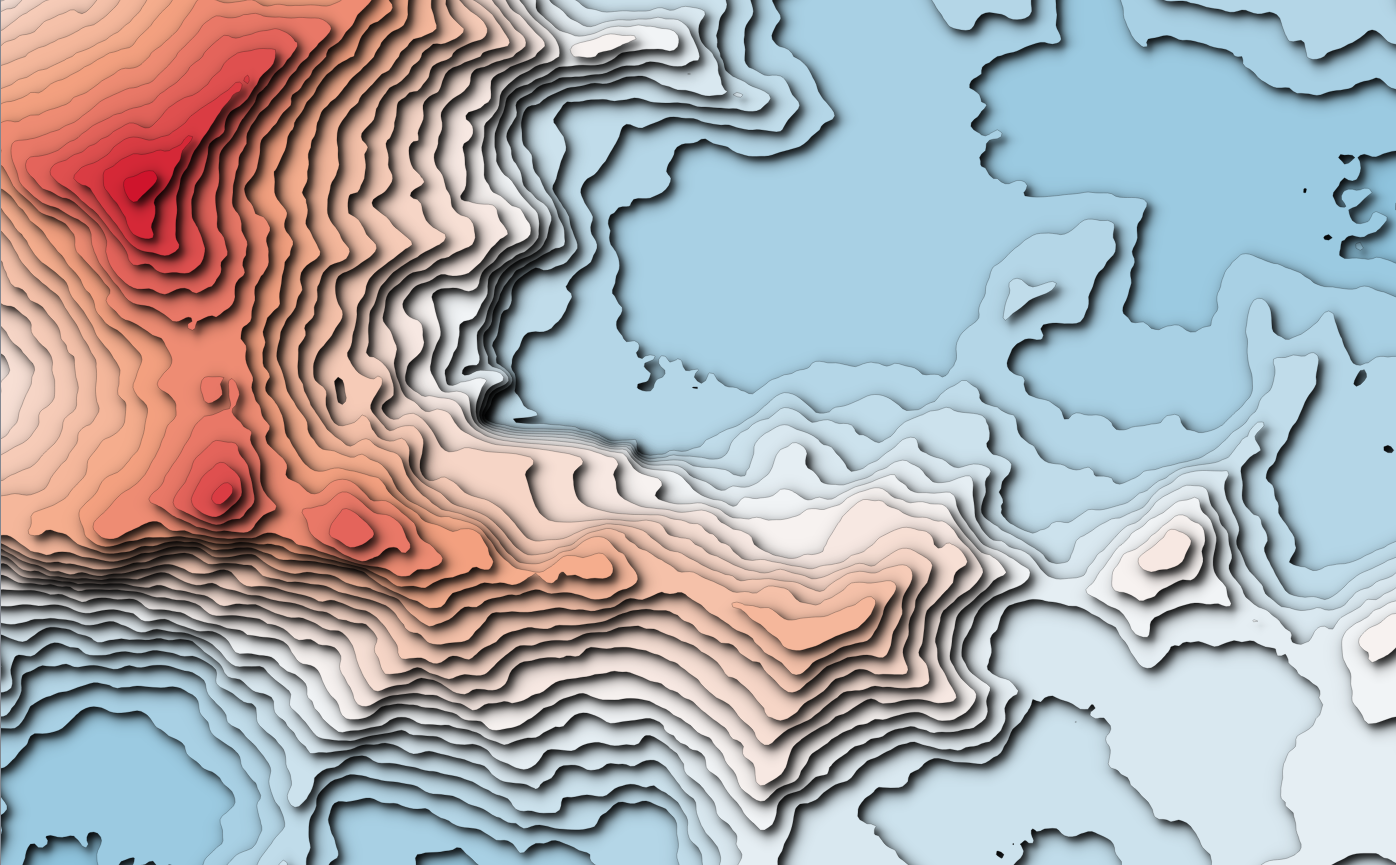
\includegraphics[width=0.2\textwidth]{test.png}
	\section{表格}
	%tabular是表格
	%{l c r}左中右对齐
	%p{1.5cm}固定宽度,自动换行
	%复杂表格搜宏包
	\begin{tabular}{l||c c c|p{1.5cm}}
		\hline \hline
		姓名 & 语文 & 数学 & 外语 & 备注 \\
		\hline
		李四 & 99 & 88 & 77 & 还行 \\
		张三 & 11 & 22 & 33 & 挂科等着换行吧 \\
		\hline
	\end{tabular}

	\newpage
	\section{浮动体}
	%浮动体参数,默认tbp
	%h,here-代码所在上下文
	%t,top -所在页面后之后页面的顶部
	%b,bottom-所在页面后之后页面的底部
	%p,page-独立一页
	浮动体的图片见图\ref{fig-dem}%引用
	\begin{figure}[htbp]
		\centering
		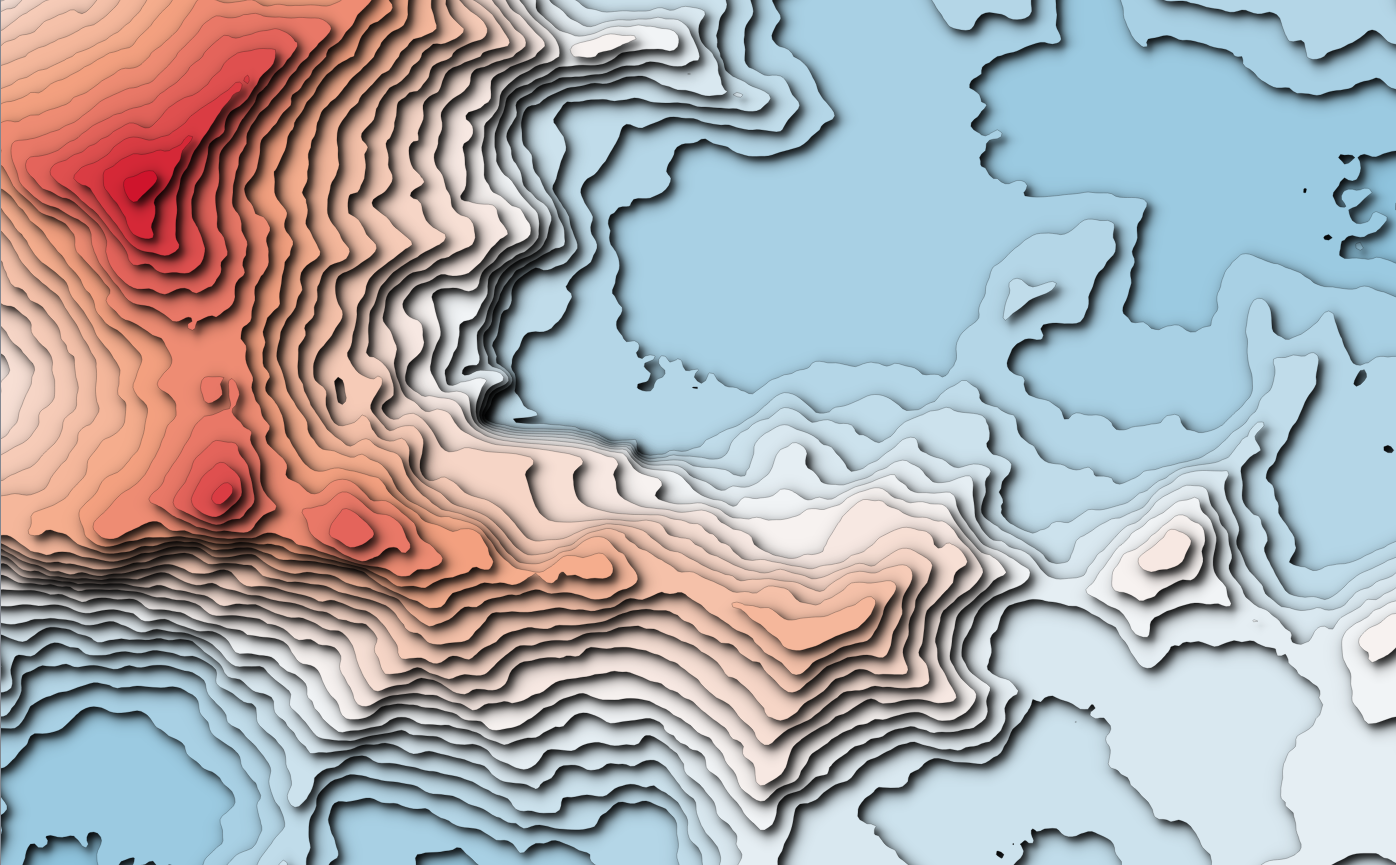
\includegraphics[height=2cm]{test.png}
		\caption{插图标题}\label{fig-dem}
	\end{figure}

	浮动体表格见表\ref{tab-score}
	\begin{table}[htbp]
			\centering
			\caption{表头文本}\label{tab-score}
			\begin{tabular}{l||c c c|r}
			\hline \hline
			姓名 & 语文 & 数学 & 外语 & 备注 \\
			\hline
			李四 & 99 & 88 & 77 & 还行 \\
			张三 & 11 & 22 & 33 & 挂科等着换行吧 \\
			\hline
			\end{tabular}
	\end{table}

	\newpage
	\section{部分公式}
	加法交换律见公式\ref{eq-change},equation加*无编号
	\begin{equation}
		a+b=b+a \label{eq-change}
	\end{equation}
	
	无定界符
	\[
	\begin{matrix}
		a & b \\
		1 & 2
	\end{matrix}
	\]
	
	小括号
	\[
	\begin{pmatrix}
		a & b \\
		1 & 2
	\end{pmatrix}
	\]
	
	中括号
	\[
	\begin{bmatrix}
		a & b \\
		1 & 2
	\end{bmatrix}
	\]
	
	大括号
	\[
	\begin{Bmatrix}
		a & b \\
		1 & 2
	\end{Bmatrix}
	\]
	
	单竖线
	\[
	\begin{vmatrix}
		a & b \\
		1 & 2
	\end{vmatrix}
	\]
	
	双竖线
	\[
	\begin{Vmatrix}
		a & b \\
		1 & 2
	\end{Vmatrix}
	\]
	
	省略号dots;ddots;vdots;还有各种省略号、行列合并、嵌套等略
	\[
	A=\begin{bmatrix}
	a_{11} & \dots & a_{1n} \\
	       & \ddots& \vdots \\
	0      &       & a_{nn}
	\end{bmatrix}_{n \times n}
	\]
	
	行内小矩阵\begin{math}
		A=\left(
		\begin{smallmatrix}
			x & y \\ w & z
		\end{smallmatrix}
		\right)
	\end{math}示例
	
	\newpage
	多行公式,加*无编号,加notag无编号
	\begin{gather}
	a+b=b+a \notag \\
	a*b=b*a
	\end{gather}
	
	多行公式对齐,\&符号指定对齐位置,也可插入多个对齐符号
	\begin{align}
		x &=t+ \cos{t}+1 \\
		xx &=2\sin{t}
	\end{align}
	
	\begin{align}
	&x =t+ \cos{t}+1 \\
	&xx =2\sin{t}
	\end{align}
	
	一个公式的多行排版
	\begin{align}
	y &=t+ \cos{t}+1 \\
	&=\cos{t+2\pi}+t+1
	\end{align}
	
	\begin{equation}
		\begin{split}
			\cos{2x}&=\cos^2{x}-\sin^2{x} \\
			        &=2\cos^2{x}-1
		\end{split}
	\end{equation}
	
	条件公式
	\begin{equation}
		sign(x)=\begin{cases}
			1, & if\ \ x>0 \\
			0, & \text{否则}
		\end{cases}
	\end{equation}
	
	
	\end{document}